\begin{thm}{068}{\hosi 4}{東大理系 (2016)}
 $z$を複素数とする。複素平面上の3点 $\mr{A}(1)$, $\mr{B}(z)$, $\mr{C}(z^2)$ が鋭角三角形をなすような$z$の範囲を求め、図示せよ。
\end{thm}

実数$a, b$を用いて、$z=a+bi$とおけば、
\[ z^2=(a+bi)^2=(a^2-b^2)+2abi \]
複素平面上の3点$\mr{A, B, C}$はそれぞれ、座標平面上の点$\mr{A}(1, 0)$, $\mr{B}(a, b)$, $\mr{C}(a^2-b^2,2ab)$に対応する。ここで、次のようなベクトルの内積を考える。
\begin{align*}
 \vvv{\mr{AB}}\cdot\vvv{\mr{AC}}&=(a-1)(a^2-b^2-1)+b\cdot 2ab \\
 &=(a+1)(a^2-2a+b^2+1) \quad\cdots\marunum{1} \\
 \vvv{\mr{BA}}\cdot\vvv{\mr{BC}}&=(1-a)(a^2-b^2-a)+(-b)(2ab-b) \\
 &=-a(a^2-2a+b^2+1) \quad\cdots\marunum{2} \\
 \vvv{\mr{CA}}\cdot\vvv{\mr{CB}}&=(1-a^2+b^2)(a-a^2+b^2)+(-2ab)(b-2ab) \\
 &=(a^2+a+b^2)(a^2-2a+b^2+1) \quad\cdots\marunum{3}
\end{align*}
これらが全て正の値をとることが、$\triangle\mr{ABC}$が鋭角三角形であることと同値である。
\[ a^2-2a+b^2+1=(a-1)^2+b^2\ge 0 \]
より、\marunum{1}から\marunum{3}が全て正の値をとることは、
\[ a+1>0 \quad\text{かつ}\quad -a>0 \quad\text{かつ}\quad a^2+a+b^2>0 \]
と同値である。
\[ a^2+a+b^2>0 \quad\dou\quad \left(a+\frac{1}{2}\right)^2+b^2>\frac{1}{4} \]
なので、求める領域は以下のようになる。
\begin{figure}[H]
 \centering
 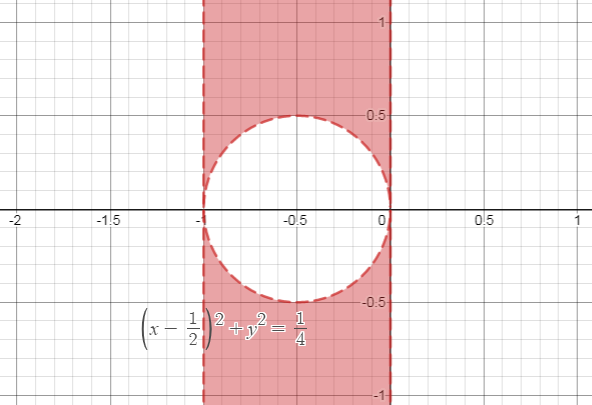
\includegraphics[width=0.7\linewidth]{../problems/Q_068/A_068.png}
\end{figure}
ただし境界は全て含まない。